\documentclass[12pt]{jbook}
% shuron.sty の漢字コードに注意
\usepackage{fancyhd,shuron}
\usepackage{graphics}
\usepackage[dvipdfm]{graphicx}
\usepackage{epsfig}
\usepackage{tabularx}
\usepackage{chapterbib}
\usepackage{makeidx}
\usepackage{amssymb}
\usepackage{url}
\usepackage{slashbox}

\makeatletter
\def\thefootnote{\ifnum\c@footnote>\z@\leavevmode\lower.5ex%
    \hbox{$^{*\@arabic\c@footnote}$}\fi}
\makeatother

\makeindex

% http://www.lab2.kuis.kyoto-u.ac.jp/~okita/etc/#0011
%%% jdummy.def
%
\DeclareRelationFont{JY1}{mc}{it}{}{OT1}{cmr}{it}{}
\DeclareRelationFont{JT1}{mc}{it}{}{OT1}{cmr}{it}{}
\DeclareFontShape{JY1}{mc}{m}{it}{<5> <6> <7> <8> <9> <10> sgen*min
    <10.95><12><14.4><17.28><20.74><24.88> min10
    <-> min10}{}
\DeclareFontShape{JT1}{mc}{m}{it}{<5> <6> <7> <8> <9> <10> sgen*tmin
    <10.95><12><14.4><17.28><20.74><24.88> tmin10
    <-> tmin10}{}
\DeclareRelationFont{JY1}{mc}{sl}{}{OT1}{cmr}{sl}{}
\DeclareRelationFont{JT1}{mc}{sl}{}{OT1}{cmr}{sl}{}
\DeclareFontShape{JY1}{mc}{m}{sl}{<5> <6> <7> <8> <9> <10> sgen*min
    <10.95><12><14.4><17.28><20.74><24.88> min10
    <-> min10}{}
\DeclareFontShape{JT1}{mc}{m}{sl}{<5> <6> <7> <8> <9> <10> sgen*tmin
    <10.95><12><14.4><17.28><20.74><24.88> tmin10
    <-> tmin10}{}
\DeclareRelationFont{JY1}{mc}{sc}{}{OT1}{cmr}{sc}{}
\DeclareRelationFont{JT1}{mc}{sc}{}{OT1}{cmr}{sc}{}
\DeclareFontShape{JY1}{mc}{m}{sc}{<5> <6> <7> <8> <9> <10> sgen*min
    <10.95><12><14.4><17.28><20.74><24.88> min10
    <-> min10}{}
\DeclareFontShape{JT1}{mc}{m}{sc}{<5> <6> <7> <8> <9> <10> sgen*tmin
    <10.95><12><14.4><17.28><20.74><24.88> tmin10
    <-> tmin10}{}
\DeclareRelationFont{JY1}{gt}{it}{}{OT1}{cmbx}{it}{}
\DeclareRelationFont{JT1}{gt}{it}{}{OT1}{cmbx}{it}{}
\DeclareFontShape{JY1}{mc}{bx}{it}{<5> <6> <7> <8> <9> <10> sgen*goth
    <10.95><12><14.4><17.28><20.74><24.88> goth10
    <-> goth10}{}
\DeclareFontShape{JT1}{mc}{bx}{it}{<5> <6> <7> <8> <9> <10> sgen*tgoth
    <10.95><12><14.4><17.28><20.74><24.88> tgoth10
    <-> tgoth10}{}
\DeclareRelationFont{JY1}{gt}{sl}{}{OT1}{cmbx}{sl}{}
\DeclareRelationFont{JT1}{gt}{sl}{}{OT1}{cmbx}{sl}{}
\DeclareFontShape{JY1}{mc}{bx}{sl}{<5> <6> <7> <8> <9> <10> sgen*goth
    <10.95><12><14.4><17.28><20.74><24.88> goth10
    <-> goth10}{}
\DeclareFontShape{JT1}{mc}{bx}{sl}{<5> <6> <7> <8> <9> <10> sgen*tgoth
    <10.95><12><14.4><17.28><20.74><24.88> tgoth10
    <-> tgoth10}{}
\DeclareRelationFont{JY1}{gt}{sc}{}{OT1}{cmbx}{sc}{}
\DeclareRelationFont{JT1}{gt}{sc}{}{OT1}{cmbx}{sc}{}
\DeclareFontShape{JY1}{mc}{bx}{sc}{<5> <6> <7> <8> <9> <10> sgen*goth
    <10.95><12><14.4><17.28><20.74><24.88> goth10
    <-> goth10}{}
\DeclareFontShape{JT1}{mc}{bx}{sc}{<5> <6> <7> <8> <9> <10> sgen*tgoth
    <10.95><12><14.4><17.28><20.74><24.88> tgoth10
    <-> tgoth10}{}
\DeclareRelationFont{JY1}{gt}{it}{}{OT1}{cmr}{it}{}
\DeclareRelationFont{JT1}{gt}{it}{}{OT1}{cmr}{it}{}
\DeclareFontShape{JY1}{gt}{m}{it}{<5> <6> <7> <8> <9> <10> sgen*goth
    <10.95><12><14.4><17.28><20.74><24.88> goth10
    <-> goth10}{}
\DeclareFontShape{JT1}{gt}{m}{it}{<5> <6> <7> <8> <9> <10> sgen*tgoth
    <10.95><12><14.4><17.28><20.74><24.88> tgoth10
    <-> tgoth10}{}
\endinput
%%%% end of jdummy.def


\begin{document}
\setcounter{page}{0}
\thispagestyle{empty}

\noindent
\includegraphics[height=2.0cm]{img/Lissajous_UEC_logo.eps}\\
\begin{tabular}{c}
{\Large 平成XX年度 修士論文}				\\
\end{tabular}

\vspace{2.5cm}

\begin{center}
\LARGE \bf 修論タイトル\\
%\vspace{4mm}
\end{center}

\vspace{1.5cm} 

\LARGE
\begin{flushright}
電気通信大学 大学院 ○○研究科\\
××専攻\\
1234567  名前\\

\vspace{1.6zh}

{\def\arraystretch{0.6}
\begin{tabular}{rll@{}}
指導教官	& ○○ ○○& 教授	\\
		& ○○ ○○& 教授	\\
		& ○○ ○○& 教授\\
							\\
提出日	& \multicolumn{2}{c@{}}{平成XX年1月30日}	\\
\end{tabular}
}
\end{flushright}
\normalsize
\newpage

\thispagestyle{empty}

\noindent
\begin{center}
\LARGE \bf 概要\\
\end{center}

\vspace{1.0cm}
{\small}
\normalsize

個人認証の安全性を高める手法として多要素認証がある.
多要素認証は,(1)知識認証,(2)所有物認証,(3)生体認証といった認証要素を複数組み合わせることで,何らかの攻撃により一つが破られても他の認証要素があることで不正利用からアカウントを守る手法である.
しかし,その普及に際しては,利便性の面から問題点がある.

本研究では,個人認証の多要素化があまり行われていない携帯端末に注目し,安全性と利便性の双方を損なうことなく,ユーザに負担の少ない多要素化手法を提案することを目的とした.

本研究では,秘密情報としてTwitterの投稿を用いた認証システムとして,(1)特定の一つを自ら選択する,(2)時系列上における期間の指定,(3)時系列上における日付と曜日の指定,の3つの秘密情報の設定方法を持ったアプリケーションソフトウェアを開発し,それぞれの設定方法について検証・評価を行った.
(1)については,秘密情報でTwitterを用いることで得られる安全性や利便性の向上について主に調査し,(2)と(3)については,ある一定のルールに基づいて秘密情報が変化することで認証の成功率やユーザへの負担がどれほど変化するかを主に調査した.

被験者実験による検証の結果,(1)については○○のような影響があり,(2)と(3)ではそれぞれ△△のような結果が得られた.
更に,考えうる問題点として××が挙げられ,具体的な解決方法についても考察した.



\newpage


\setcounter{page}{1}

% 目次
\tableofcontents
% 図目次
\listoffigures
% 表目次
\listoftables

% 論文本体
%序論背景と目的
\chapter{序論}\label{chap:introduction}
\section{背景}
通信網の高速化・大容量化,電子機器の小型化・高性能化などにより,Webサービスで可能なことが多くなった.
また,高性能な携帯端末の普及により,個人や決済にかかわる重要な情報を持ち歩くことが一般化しつつあり,必然的に個人認証を行う場面が増えてきている.
こういった場面における個人認証では,パスワードや暗証番号\footnote{本論文において暗証番号認証は,特に指定がない限り 4 桁の数字を秘密情報としたものを想定する.}(英語ではPersonal Identification Number (略称: PIN))を用いた例をよく見かける.

特にパスワードを用いた認証では,安全性と記憶持続性・利便性に関してはトレードオフの関係が存在する.
例えば,辞書攻撃に強い安全なパスワードを用いようとする際には,意味のない文字列にすることが望ましい.
しかし,意味のない文字列というのは覚えることが難しく,ユーザがパスワードを他のサービスにおいても使い回してしまう可能性が高まり,どれか一つのサービスからパスワードが流出した際,かえって脆弱になってしまう恐れがある.
現在,こういった問題を防ぐものとして,多要素認証を自由意志で利用できるWebサービス(Google\cite{google},Dropbox\cite{dropbox}やEvernote\cite{evernote}など)が増加しつつある.
例えば,パスワードの入力が完了し,それが正しいものだと判断された後に,あらかじめ登録された電話番号にSMS(Short Message Service\footnote{電話番号を利用して短いメッセージを送受信できるサービス})を利用してワンタイムパスワードを送信し,それを入力させるといった方式をとることができる.
これにより,覗き見,推測や総当り攻撃によってパスワードが漏洩した際の不正利用のリスクを減少させることが可能となる.
多要素認証を何らかの方法で適用する行為を個人認証の多要素化と定義する.

また,Social Networking Service\footnote{Social Networking Service,社会的ネットワークをインターネット上で構築するサービス.}(以下,SNS)の形態を持つWebサービスが近年増えてきている.
これにより,コミュニケーションの道具やライフログとして自分自身の情報を公開することが多くのユーザ間で一般的になりつつある.
SNSにおいては,公開範囲をある程度任意に指定できるサービスが多いという特徴がある.

\section{研究目的}
本研究における目的は,SNSの情報を用いて記憶持続性と利便性に考慮しつつ個人認証の安全性を向上させることである.
現在行われている個人認証の多要素化は,セキュリティトークンやEメールを用いたものが一般的であり,それにより大きく認証の安全性を高めている.しかし,利便性という点においては,一度認証のための画面から目を逸らす必要がある,特別なハードウェアを持ち歩く必要があるなど,今後の普及に際して改善の余地があると考えられる.

本研究ではSNSの情報を用いた個人認証の提案が少ないことに着目し,応用可能な例として携帯端末に搭載することを想定したシステムを考案した.

\newpage

\section{論文の構成}
本論文は以下の章により構成される.\\
\\
第 \ref{chap:introduction} 章 序論:この章では,本研究を行うに至った背景と主たる目的に関する解説を行う.\\
第 \ref{chap:preparation} 章 個人認証の多要素化への流れ:この章では,認証技術の現状や,個人認証へ及ぼすと考えられる影響について述べる.\\
第 \ref{chap:relatedwork} 章 関連研究/製品:この章では,前章で述べた内容に関連する,既存の製品や研究の取り組みを紹介する.\\
第 \ref{chap:motive} 章 動機と提案:この章では,既存の認証における問題点と,それを改善するために近年普及した技術やサービスを用いる理由と既存手法,更に提案手法の概要について説明する.\\
第 \ref{chap:system} 章 Twitter上の情報を用いた認証システム:この章では,本研究で開発したシステムに関する原理と詳細説明を行う.\\
第 \ref{chap:experiment} 章 検証実験:この章では,本研究で開発したシステムを用いた実験についての内容と結果の説明を行う.\\
第 \ref{chap:discussion} 章 考察:この章では,これまでの取り組みと得られた結果から,本研究の成果と各結果に対する考察,ならびに今後の課題について考察する.\\
第 \ref{chap:conclusion} 章 結論:この章で本研究について総括する.\\

\newpage


%関連研究
\chapter{個人認証の多要素化への流れ}\label{chap:preparation}

\section{既存の認証技術}
一般に認証手法は以下の3つに大別できる.

\subsection{知識認証}\label{subsec:knowledge}
本人のみが記憶している情報を秘密情報として認証を行う手法.
主にキーボードやタッチパネルなどの入力インターフェースを用いてアウトプットを行う.
この手法は他の認証方式と比較して以下のようなメリットから,一般のWebサービスやモバイル端末などにおける認証に多く普及している.
\begin{itemize}
\item 多くの端末に搭載される汎用的な入力インターフェースを利用できるため,実装される環境への依存が少ない
\item 新たなハードウェアを必要とする場面が少ないため,低コストで導入できる
\item 秘密情報の伝達や保管が容易
\end{itemize}
秘密情報として,パスワード(図\ref{fig:loginGoogleWithIDAndPass})やPIN(図\ref{fig:iosPIN})が用いられることが多い.
そのため,以下のような欠点が存在する
\begin{itemize}
\item ユーザへ強いる記憶負担が大きい
\item 認証のための秘密情報入力に際して負担が大きい
\item 情報量が少なく,総当り攻撃や辞書攻撃に対して脆弱
\end{itemize}
推測が難しいパスワードにするには意味を持たせないほうがよいため,記憶するのが難しくなりがちである.
しかし,ユーザにそういったパスワードを使用させることは難しく,Ashlee Vance\cite{21password}によれば,パスワードの20\%がわずか5000個のリストで網羅可能である.

\begin{figure}[th]
\begin{center}
\epsfig{file=img/loginGoogleWithIDAndPass.eps,scale=0.50}
\end{center}
\caption{Google におけるIDとパスワードの入力画面}
\label{fig:loginGoogleWithIDAndPass}
\end{figure}

\begin{figure}[th]
\begin{center}
\epsfig{file=img/iosPIN.eps,scale=0.25}
\end{center}
\caption{Aplle iOS におけるタッチパネルによるPINの入力画面}
\label{fig:iosPIN}
\end{figure}

\subsection{所有物認証}\label{subsec:possession}
本人のみが所有している物の情報を秘密情報として認証を行う手法.
他の認証手法に対して,
\begin{itemize}
\item 入力においてユーザの負担が少ない
\item 所有物を交換することで秘密情報を容易に変更可能
\item 秘密情報の情報量を増やしやすいため,比較的容易に安全性を高められる
\item 貸与が可能
\end{itemize}
などの利点がある.しかしながら,
\begin{itemize}
\item 認証に際してその場に所有していることが求められるため,ユーザの負担が大きい
\item 認証に特殊な機器を必要とするため,導入のコストが高い
\item 盗難・紛失した場合,容易になりすましされる恐れがある
\end{itemize}
といった欠点も抱えている.
具体例としては,IDカードやUSBキー(図\ref{fig:dongle}),ハードウェアトークンを用いたワンタイムパスワードによる認証などが挙げられる.

\begin{figure}[th]
\begin{center}
\epsfig{file=img/dongle.eps,scale=0.50}
\end{center}
\caption{USBキーの例}
\label{fig:dongle}
\end{figure}


\subsection{生体認証}\label{subsec:inherence}
本人の生体情報を秘密情報として認証を行う手法.
\begin{itemize}
\item 所有物認証のように何かを持ち歩く必要がなく,盗難・紛失の恐れも少ないため,ユーザへの管理負担が少ない
\item 入力においてユーザの負担が少ない
\item 秘密情報の情報量が大きい
\end{itemize}
などの利点を持つ反面,
\begin{itemize}
\item 秘密情報の変更が困難
\item 認証に特殊な機器を必要とするため,導入のコストが高い
\item 盗難・紛失した場合,容易になりすましされる恐れがある
\item 体質や外部からの影響により認証操作を行うことが困難な場合がある.
\end{itemize}
などの欠点が存在する.
この認証方式の具体例として,指紋・静脈(図\ref{fig:veinAuth})・虹彩を用いたものが挙げられる.

\begin{figure}[th]
\begin{center}
\epsfig{file=img/veinAuth.eps,scale=0.5}
\end{center}
\caption{静脈を用いた認証のための装置}
\label{fig:veinAuth}
\end{figure}

\section{多要素認証}\label{sec:2factor}
既存の認証手法を複数提供し組み合わせることで,欠点を補い,安全性を高めることができる.
これが多要素認証である.
個人認証の多要素化の実現においては,ワンタイムパスワードを要素の一つとして利用している方式が主流である.\cite{arXiv:1309.5344}

銀行/オンラインゲームなどで多く見られるのが,ハードウェアトークンと呼ばれる,ワンタイムパスワード生成器を用いた方式である.

さらに近年,GoogleやFacebook,Appleなど,多くの金融にかかわらないWebサービスでは,パスワードを保持するデータベースの増加とその認証情報の流出による,パスワードリスト型攻撃へのリスクを緩和するために多要素認証を用意している.
そういったサービスで利用される方式として,SMS/Eメールやスマートフォン\footnote{インターネットの利用を前提とした高機能携帯電話.統一された定義はないが,一般社団法人 情報通信ネットワーク産業協会によれば「携帯電話・PHSに携帯情報端末(PDA)を融合させた端末で、音声通話機能・ウェブ閲覧機能を有し、仕様が公開されたOSを搭載し、利用者が自由にアプリケーションソフトを追加して機能拡張やカスタマイズが可能な製品。」(出展:通信機器中期需要予測 2010年度 CIAJ)} 用アプリケーションを用いたものがある.
SMS/Eメールを用いた際は,手持ちの携帯端末に乱数が記載されたメッセージが送信され,アプリケーションを用いた場合は,アプリケーション上に乱数が表示される.
この方式のメリットとして,新たなハードウェアを持ち歩く必要がなくなることによる利便性の向上と,併せて紛失の危険性も減少するということが挙げられる.

多要素認証のデメリットとしては,
\begin{itemize}
\item 中間者攻撃やトロイの木馬を用いた攻撃,フィッシングに対して弱い
\item サービスプロパイダが負担するコストが大きい
\end{itemize}
などが挙げられる.

実例としての多要素化手法やワンタイムパスワードの生成方式については,第\ref{chap:relatedwork}章で述べる.

\section{スマートフォン/タブレットの普及}
2013年6月に行われたIDC Japanの調査\cite{idcsmartphone}によれば,家庭市場におけるスマートフォンの所有率は49.8\%,タブレット\footnote{板状のオールインワン・コンピュータやコンピュータ周辺機器の総称.本論文では,特に断りがなければ携帯端末としてのタブレットを指す.}の所有率は20.1\%であった.
これらの携帯端末の普及により,外出先などからも様々なサービスにアクセスすることが可能になった.
しかしその反面,様々なサービスの認証情報や個人情報などのデータを外に持ち出している状態であるため,携帯端末のセキュリティをいかに強化するかが重要になってきている.

スマートフォン/タブレットでは,携帯端末専用又はタッチパネルなどによる操作に特化したOS\footnote{Operating System,基本ソフトとも.ハードウェアを抽象化しインターフェースを提供するソフトウェア}が搭載されていることが多く,Webサービスなどにおいても,ブラウザ上からだけでなく,専用のアプリケーションソフトウェアが用意されている場合がある.
そういった場面では,認証情報は端末内に保存され,毎回の個人認証操作を行う必要が省かれていることもあり,端末の画面ロック\footnote{操作を大きく制限されている状態.PIN認証などを行わない限り解除できないことが一般的である.}が解除されてしまえば,従来の携帯電話などと比較して多くの操作が可能になってしまう.

携帯端末は,\ref{sec:2factor}章や\ref{sec:multifactor}章で述べられているように,多要素認証における認証要素の一つとしても扱われている現状が存在する.

\section{Social Networking Serviceの普及}
2011年の総務省の調査\cite{micwhitepaper24}では,成人におけるSocial Networking Service(以下SNS)の利用率は15.0\%であり,この数字は年々増加傾向にある.SNSでは,多くのユーザがコミュニケーションやライフログを行うために投稿を行っている.そのため,個人を特定するための情報が多く存在するといえる.

SNS上の情報は公開範囲を定めることができるという特徴を持つ.
全世界に公開されるパブリックなものから友人のみが閲覧可能な情報や,自分のみが見ることができるプライベートな情報を発信できる.

SNSの一つにTwitterというサービスがある.
これはユーザが個人で短文(140字以内)を投稿する,ミニブログやマイクロブログといったカテゴリーに分類されるのものである.
Twitter上の情報はほとんどがタイムライン\footnote{投稿が時系列によって表示される画面}に表示される短文の投稿(「ツイート」と呼ばれる)であり,それら自体に単独で公開範囲を定めることはできないが,アカウントがprotected(一般非公開の状態)に設定されていれば,フォロー\footnote{他ユーザの投稿を自分のタイムラインで表示できるよう登録すること}を許可された人物(フォロワー\footnote{自分のことをフォローしている他のユーザ})のみが閲覧できる状態になる.
アカウントがパブリックであれば,自分の投稿は他のユーザが自由に閲覧できる.しかし,他人への返信は自分と相手の共通のフォロワーでないとタイムライン上には表示されない.
Twitterでは以上のようにパブリックとprotectedの2つの公開範囲が存在する.
\newpage

%関連研究
\chapter{関連研究}\label{chap:relatedwork}

こんなんのもありまっせ.
\ref{chap:introduction}章にも書きましたぜ.

\section{Aの関連研究}
\label{sec:relatedworkA}

\ref{subsec:ura}節に、本研究の真の目的を書いたが、その理由はこの関連研究にある.

\newpage

%理論と仮説
\chapter{動機と提案}\label{chap:motive}
\section{動機}\label{sec:motive}
ここまでの章で多要素認証の現状について述べてきたが,今後の普及に向けて解決しなければならない問題点:(1)コストと(2)利用可能な状況,がある.

(1)コストについては2つの見方がある.
1つはサービス提供側が負担しなければならないコストであり、もう1つは利用者が負担しなければならないコストである.
そのそれぞれについて以下に述べる.
\begin{itemize}
  \item サービスプロバイダは,多要素認証の導入のために新たなハードウェアトークンや認証用機器,新たなシステムを用意する負担を強いられる
  \item ユーザは,ハードウェアトークンを管理・携帯したり,認証を行う際に携帯端末の画面を確認しなければならないといった負担を強いられる
\end{itemize}
上記のように,現状では双方にとってあまり手軽とは言えない.
そのため,導入を妨げないようなシステムを提案することが普及の鍵になると考えた.

また,(2)利用可能な状況に関しても,ワンタイムパスワードのSMS/Eメールを用いた送信や携帯端末を用いた生成は,ネットワークに接続していて操作の権限を持つ端末が必要であるし,そもそも個人で使える多要素認証はWebに関わるものが多く,そうではない場面,例えば携帯端末そのものの認証やオフラインな状況でも使える多要素化の方法を模索する必要があると考えた.

\subsection{携帯端末への多要素認証の導入}
スマートフォン/タブレットでは,携帯端末専用又はタッチパネルなどによる操作に特化したOS\footnote{Operating System,基本ソフトとも.ハードウェアを抽象化しインターフェースを提供するソフトウェア}が搭載されていることが多く,それらは高機能な開発環境が公開されている.
そのため,Webサービスなどにおいても,専用のアプリケーションソフトウェアがサービスプロバイダによって用意され,ブラウザ上からアクセスする必要がなくなりつつある.
そういった場面では,認証情報は端末内に保存され,毎回の個人認証操作を行う必要が省かれていることもあり,端末の画面ロック\footnote{操作を大きく制限されている状態.PIN認証などを行わない限り解除できないことが一般的である.}が解除されてしまえば,従来の携帯電話などと比較して多くの操作が可能になってしまう.
以上の理由から,携帯端末のセキュリティを向上させることが必要であり,その際に多要素認証を適用できるのではないかと考えた.

更に,それぞれのアプリケーション(例:写真アルバム,メモ,ブラウザなど)に対して,プライバシーを保護するためにロックをかけたいといった需要が存在し,そのためのソフトウェアも既に開発されている(\ref{subsec:passboard}など).
そういった場面で気軽に安全性を強化できる新たなアイデアとしても提案できないかと考えた.

\section{提案}
本論文では,個人認証における利便性を
\begin{description}
  \item[覚えやすさ] 秘密情報を覚えて認証を行うまでの期間記憶保持することの肉体的・精神的・時間的負担の少なさ
  \item[使いやすさ] 認証及び秘密情報設定の際の肉体的・精神的・時間的負担の少なさ
\end{description}
の2指標で定義する.
個人認証の方法を提案するにあたって,認証の強度を高めることによって利便性を損ねてしまうことは避けなければならない.
そこでライフログ\footnote{人間の行いをデジタルデータとして記録する技術・行為.ブログやSNSの一部などもライフログだといえる.}は個人の生活や行動,体験などに基づいているため,個人を特定できる要素が多く,しかも記憶持続性が高いという想定から,個人認証と親和性が高いのではないかと考えた.

また,写真,動画,音楽などの共有(Instagram)や買い物(Amazon.co.jp)などWebサービスで行えることが増えてきているが,その中でもSNSは2011年の総務省の調査\cite{soumuWhitepaper2013Social}では52.9\%が1回以上利用したことがあるとされており,若年層ほど利用率が高く,10代と20代ではそれぞれ71.7\%と63.9\%が現在継続して使用しているという結果が明らかになった.
SNS上の情報は,全世界に公開されるパブリックなものから友人のみが閲覧可能な情報や,自分のみが見ることができるプライベートな情報まで,様々な公開範囲を定めて発信できるという特徴を持つ.
この特徴は,秘密情報の候補として認証時に表示してもよいものが得られるため,情報漏洩などの被害を抑えることができるのではないかと仮定した.

これらの技術を用いることで,強度と利便性を兼ね備えた認証を提案できないかと考えた.

\subsection{ライフログやSNSを利用した個人認証事例}\label{sec:lifeLogAuth}
ライフログやWebサービスを用いた認証について,5つの既存手法を紹介する.

\subsubsection{Web履歴を用いた認証}\label{subsec:webHistoryAuth}
田村ら\cite{田村健範:2011-07-14}は,Webに頻繁に接続するユーザである場合,閲覧履歴を用いて``平日の平均Web接続時間'',``平日,休日のアクセスドメイン''によってユーザの特徴を抽出できる可能性があるとした.その際は本人認証をWeb閲覧履歴のみによって行えるが,Webに頻繁に接続しないユーザの場合は,ユーザを識別できるほどの特徴が見いだせないという結果が得られている.また,複数のライフログを用いた多要素化についても述べられている.
問題点として,本人の趣味趣向を真似ることによってなりすましが行いやすいことが挙げられる.

\subsubsection{GPSを用いた認証}\label{subsec:gpsAuth}
長谷ら\cite{長谷容子:2004-08-20}は,ユーザがあらかじめ予定していた時間に,予定していた場所へ移動したかどうかの情報を個人認証のための特徴量として扱う検討を行った.これによれば,複数のチェックポイントを設け,その場所で送信されたGPSデータを到着予定場所のものと比較することで,個人認証を行える可能性があるとしたが,GPSデータの送信が不可能な場所や,予定時刻へ間に合わない場合が存在するなどの問題点が存在することも示した.

また,今澤ら\cite{imazawa:2008-10-08}は,GPSデータからユーザが滞在していた場所と時刻の情報を抽出し,ユーザに停留点を回答させる手法で,認証システムを実装した.これによれば,ユーザの1週間の停留点数が10点以下であった場合に選択肢が減少し安全性が損なわれてしまう可能性があるが,必要操作や依存環境の少なさから様々な場面で応用できるとした.
更なる問題点として,GPSのデータを逐一送信できないと認証の安全性が確保しにくくなることが挙げられる.

\subsubsection{電子メールを用いた認証}\label{subsec:emailAuth}
西垣ら\cite{西垣正勝:2006-03-15}は,ユーザの生活履歴を用いて認証を行う手法を提案し,そのプロトタイプとしてEメールを用いたシステム(図\ref{fig:nishigakiMail})の構築と実験を行った.Eメールによる認証は,「最近のメールかどうか」をユーザに回答させるというプロセスで行われた.その際,人間の記憶の曖昧性を取り除くための手法として$ ( n + 1 ) $日前から$ ( m - 1 ) $日前までのメールは認証に使用しないように設定し,最近と過去どちらともいえないような期間のメールを利用しない:例えば$ n = 7 $,$ m = 30 $とすることで「8日前から29日前までのメールは質問の中に出てきません」と明示することでユーザが直感的に回答を行えるようにする,という工夫がなされた.
さらに,基礎実験の後に「最近のメール」といった選択肢に加え「曖昧だが最近のメール」といった曖昧な回答の選択肢を追加することで,重要でない故に記憶に残っていないメールを認証に使用しないようにするという改善策をとった結果,最終的に本人による認証では99\%の正答率を得た.
問題点として,重要であったりプライベートなメールが認証時に表示されてしまうことで,情報漏洩やプライバシー情報流出の可能性がある.

\begin{figure}[ht]
  \begin{center}
    \includegraphics[width=140mm]{img/nishigakiMail.pdf}
  \end{center}
  \caption{電子メールを用いた認証のシステム}
  \label{fig:nishigakiMail}
\end{figure}

\subsubsection{TwitterのDirect Messageを用いた認証}\label{subsec:twitterDMAuth}
Nemotoら\cite{nemoto:2006-03-15}は,Twitterのダイレクトメッセージ\footnote{特定のユーザ宛に,一対一で送信された文章のこと.閲覧可能な人物は,自分と相手のみである.}(DM)機能を用いて,定期的に質問を投げかけることでその回答を秘密情報とし,認証を行うシステム,KBA\footnote{Knowledge-Based Authentication}(図\ref{fig:twitterNemoto})を提案した.
質問の内容は「2月15日の昼食は?」といった文面で構築され,Twitterのダイレクトメッセージ機能により送信され,回答も同機能を用いて行う.
この手法は,メッセージ機能を用いて秘密の質問を定期的に更新しているだけで,SNS上でそれを実行する必要性が希薄であると考えられる.

\begin{figure}[ht]
  \begin{center}
    \includegraphics[width=140mm]{img/twitterNemoto.pdf}
  \end{center}
  \caption{TwitterのDirect Messageを用いた認証のシステム}
  \label{fig:twitterNemoto}
\end{figure}

\subsubsection{友人の顔写真を用いた認証}\label{subsec:facebookFaceAuth}
Facebook\footnote{米Facebook社が提供しているSNSである.本名での登録が必須という特徴を持つ.2004年に学生のみが使用できるサービスであったが,その後一般にも開放され,現在では世界最大のアクセス数を誇るSNSとなっている.}では,友人の顔写真を用いた個人認証が運用されている.認証手法は,顔写真が質問として提示され,これに対してその人物の本名を回答する方法である.
これはパスワードを忘れてしまった際や,アカウントへの不審なアクセスが確認された場合の本人証明に使われている.
Facebookにはユーザから投稿された写真にユーザ名を結びつけることができ,さらに自動で人の顔を抽出しタグ付けを行う機能も存在するため,そういった情報を利用していると考えられる.
欧州ではプライバシー保護のためこの自動顔認識の機能が無効にされるなどしている.
更なる問題点として,友人が自分の顔にのみタグ付けしているという保証がなく(他の動物や物体にも名前のタグ付けが可能),その場合答えられないという状況が発生し得ることが挙げられる.

\begin{figure}[ht]
  \begin{center}
    \epsfig{file=img/facebookFaceAuth.eps,scale=0.5}
  \end{center}
  \caption{Facebookにおける友人の顔写真を用いた認証画面}
  \label{fig:facebookFaceAuth}
\end{figure}

%\section{既存システムの問題点}
%既存のライフログを用いた認証方式の問題点として,
%\begin{enumerate}
%  \item 本人の趣味趣向を真似ることによってなりすましが行いやすい(Web履歴を用いた認証)
%  \item GPSのデータを逐一送信できないと認証の安全性が確保できない(GPSを用いた認証)
%  \item 重要であったりプライベートなメールが認証時に表示されてしまうことで,情報漏洩やプライバシー情報流出の可能性がある(電子メールを用いた認証)
%  \item メッセージ機能を用いて秘密の質問を定期的に更新しているだけで,SNS上でそれを実行する必要性が希薄である(TwitterのDirect Messageを用いた認証)
%  \item 友人が自分の顔にのみタグ付けしているという保証がなく(他の動物や物体にも名前のタグ付けが可能),その場合答えられないという状況が発生しうる(友人の顔写真を用いた認証)
%\end{enumerate}
%などが挙げられる.

\subsection{提案手法の概要}
前節の各既存手法の問題点を,3つに大別する.
\begin{description}
  \item[特定の攻撃手法に対して脆弱になりうる状況が存在するもの] Web履歴を用いた認証,GPSを用いた認証
  \item[認証時に表示される情報に問題があるもの] 電子メールを用いた認証,友人の顔写真を用いた認証
  \item[利便性について提案以前の状態から改善できていないもの] TwitterのDirect Messageを用いた認証
\end{description}

その上で提案手法によって目指すべき点をまとめると以下のようになる.

\begin{enumerate}
  \item 従来の多要素認証方式に存在した,以下の問題点を解消する
  \begin{enumerate}
    \item 導入に際してかかる金銭的・精神的なコストや負担といった問題点を,既存の入力手法を用いることで解消できる可能性がある
    \item ハードウェアやネットワークへの依存し,導入のための状況が限られるという問題点を,予め保存できる知識情報を用いることで改善できる可能性がある.
  \end{enumerate}
  \item 能動的に発信した文章を秘密情報として使用することで,従来の知識認証において利用者の負担となっていた記憶負担を低減できる可能性がある
  \item 前節で述べた既存の認証方式に存在した,以下の3つの問題点を解消する
  \begin{enumerate}
    \item 特定の趣向や環境に依存してしまうと,一部の攻撃手法に対して脆弱になったり,エントロピーの問題から認証の安全性を担保できないことがあるため,雑多な自分自身の投稿を用いることでそれらの依存を解消できる可能性がある
    \item 認証時に表示される情報が,認証とは別に攻撃者に見られては困るものである場合を禦ぐため,既に公開情報となっている自分の投稿を用いることで,安全性の中でも特にプライバシー面での問題を解消する
    \item 定期的に秘密情報に関する質問が行われるなど,利便性の面から大きく改善が見られないため,自分が日常的に行っている投稿から秘密情報をつくりだすことで,能動的に覚える作業や定期的な更新の必要性を減らせる可能性がある.
  \end{enumerate}
\end{enumerate}

以上の問題点と解決方法によって,従来の方式に比べて
\begin{itemize}
  \item 利便性
  \item 安全性
\end{itemize}
をどちらも損なわず両立させた個人認証手法を目指した.


%システム
\chapter{Twitter上の情報を用いた提案認証システム}\label{chap:system}
\section{既存システムの問題点}
既存のライフログを用いた認証方式の問題点として,
\begin{enumerate}
\item 本人の趣味趣向を真似ることによってなりすましが行いやすい(Web履歴を用いた認証)
\item GPSのデータを逐一送信できないと認証の安全性が確保できない(GPSを用いた認証)
\item 重要であったりプライベートなメールが認証時に表示されてしまうことで,情報漏洩やプライバシー情報流出の可能性がある(電子メールを用いた認証)
\item メッセージ機能を用いて秘密の質問を定期的に更新しているだけで,SNS上でそれを実行する必要性が希薄である(TwitterのDirect Messageを用いた認証)
\item 友人が自分の顔にのみタグ付けしているという保証がなく(他の動物や物体にも名前のタグ付けが可能),その場合答えられないという状況が発生しうる(友人の顔写真を用いた認証)
\end{enumerate}
などが挙げられる.

\section{採用手法の概要}
前節の問題点するためには,それらを3つに大別した上でそれぞれについて以下のような改善策を用意できると考えた.
\begin{itemize}
\item 安全性が損なわれる状況が存在する(1,2):特定の趣向や環境に依存しにくい情報を利用する
\item 認証時に問題が生じる(3,5):ある程度公開されている情報を用いたり,イレギュラーをフィルタリングしやすいように文字情報を主として用いる
\item 利便性について提案以前の状態から改善できていない(4):能動的に憶えるのではなく,憶えていることを認証に利用する
\end{itemize}
そして提案システムではSNSの情報,今回はTwitter上にある自分のツイートを利用することで上記の改善策を取り入れることができると考えた.
積極的理由として,
\begin{enumerate}
\item 能動的な行為によって生成される情報であり,記憶のための負担に配慮可能なこと
\item 生成された日時の詳細が確実に取得でき,時系列を提示することにより記憶を思い出しやすいこと
\end{enumerate}
が挙げられ,他にも考えうる手段としては以下の様なものがあったが,記載の理由により前述の手法をとることにした.
\begin{itemize}
\item 音楽を用いて認証を行う方法:認証を行いにくい場面が存在すること,趣味趣向に大きく依存してしまうこと
\item Twitterのお気に入り情報を用いる手法:お気に入りに登録された日時が取得できないこと,お気に入りにしたツイート自体は他人の制御下にあるため
\end{itemize}

また,時系列における情報を保持していることの特徴として,時間情報によって範囲を指定することで,秘密となる情報群を抽出することができるというものがある.
また,相対的な時間情報の指定を行うことで秘密情報の対象を自動で入れ替えることが可能となる.
これによる具体的な利点は\ref{sec:feature}節にて示す.

\section{システムの詳細}
本論文における提案システムとして,前節の内容を踏まえて,利便性(憶えやすさ/使いやすさ)と安全性の両立を目指した個人認証手法を実装した(以下Notifauth).
Notifauth起動時の画面は図\ref{fig:notifauthHome}のようになっており,この画面から新規登録画面(図\ref{fig:notifauthLogin})\footnote{Twitterと連携するためOAuthを用いた}への遷移,設定画面への遷移,実験の試行を開始,実験結果の送信を行うことが可能となっている.

\begin{figure}[ht]
\begin{minipage}{0.5\hsize}
\begin{center}
\includegraphics[width=60mm]{img/notifauthHome.eps}
\end{center}
\caption{Notifauth起動時の画面}
\label{fig:notifauthHome}
\end{minipage}
\begin{minipage}{0.5\hsize}
\begin{center}
\includegraphics[width=60mm]{img/notifauthLogin.eps}
\end{center}
\caption{Notifauthユーザ登録画面}
\label{fig:notifauthLogin}
\end{minipage}
\end{figure}

\subsection{秘密情報の設定}
この手法を用いた秘密の設定方法として,
\begin{itemize}
\item Auto Mode Type Term:○日/週/月/年前から△日~年間を指定し,認証時点にその範囲に当てはまるツイートが秘密情報となる(図\ref{fig:notifauthAutoTerm})
\item Auto Mode Type Cycle:○曜日の△時台という条件に当てはまるツイートが秘密情報となる(図\ref{fig:notifauthAutoCycle})
\item Manual Mode:自分のツイートから任意に1つ秘密情報となるものを選ぶ(図\ref{fig:notifauthManual})
\end{itemize}
以上の3つを実装した.

\begin{figure}[ht]
\begin{minipage}{0.5\hsize}
\begin{center}
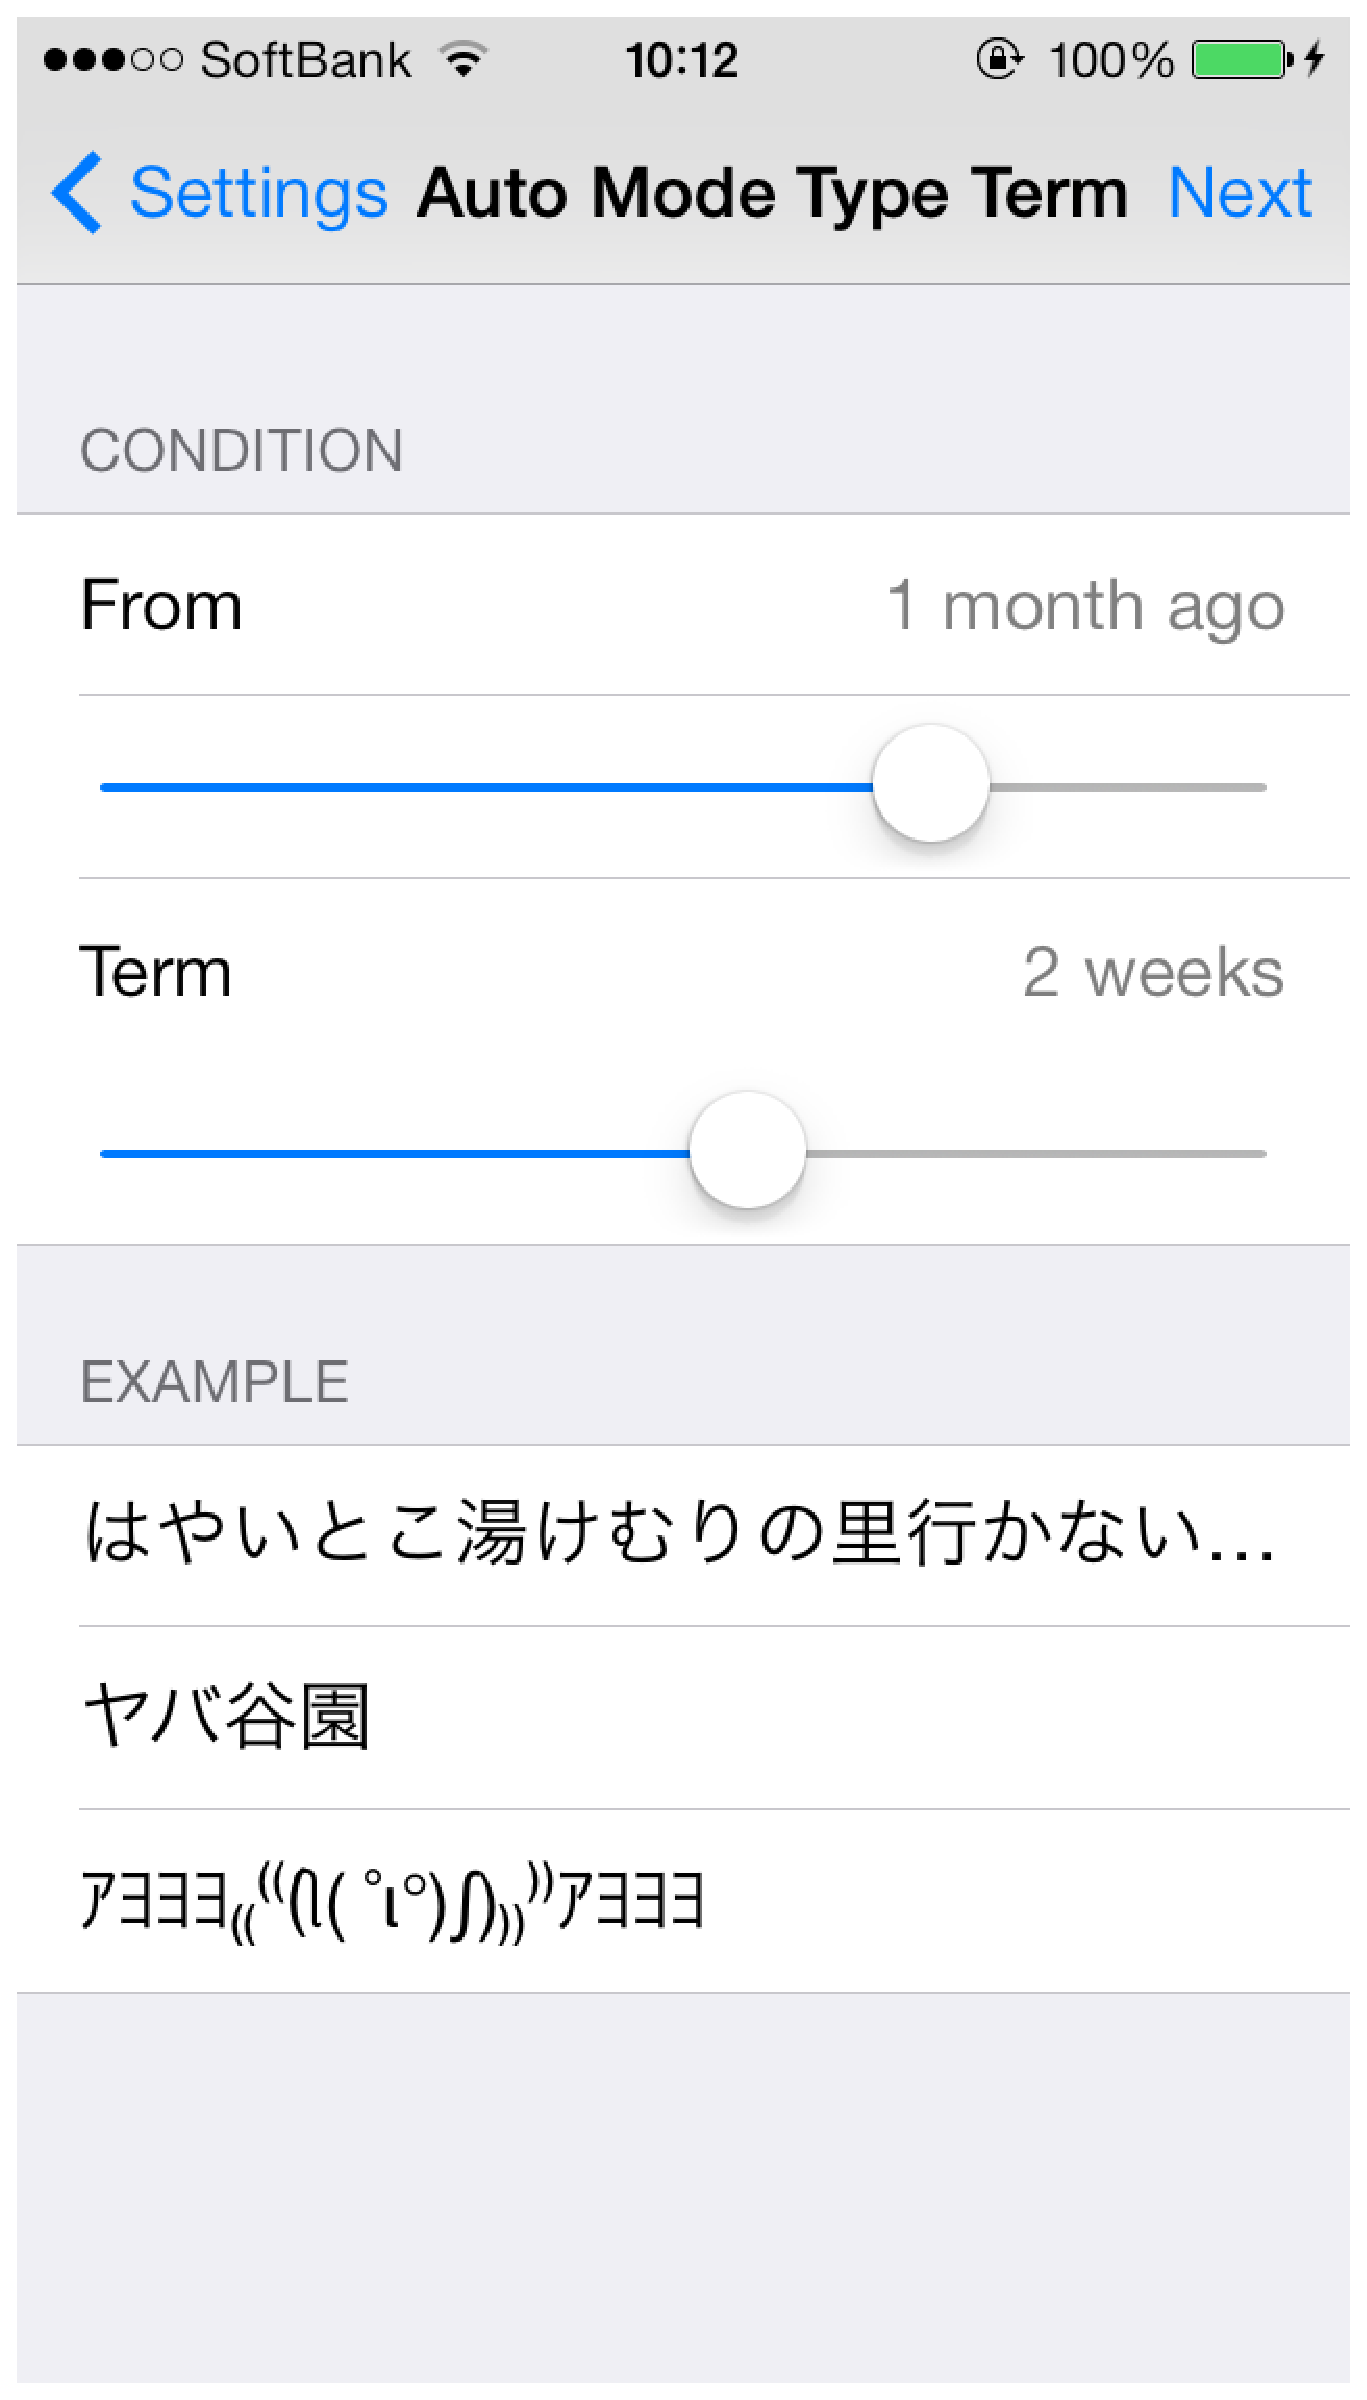
\includegraphics[width=60mm]{img/notifauthAutoTerm.eps}
\end{center}
\caption{Auto Mode Type Termの設定画面}
\label{fig:notifauthAutoTerm}
\end{minipage}
\begin{minipage}{0.5\hsize}
\begin{center}
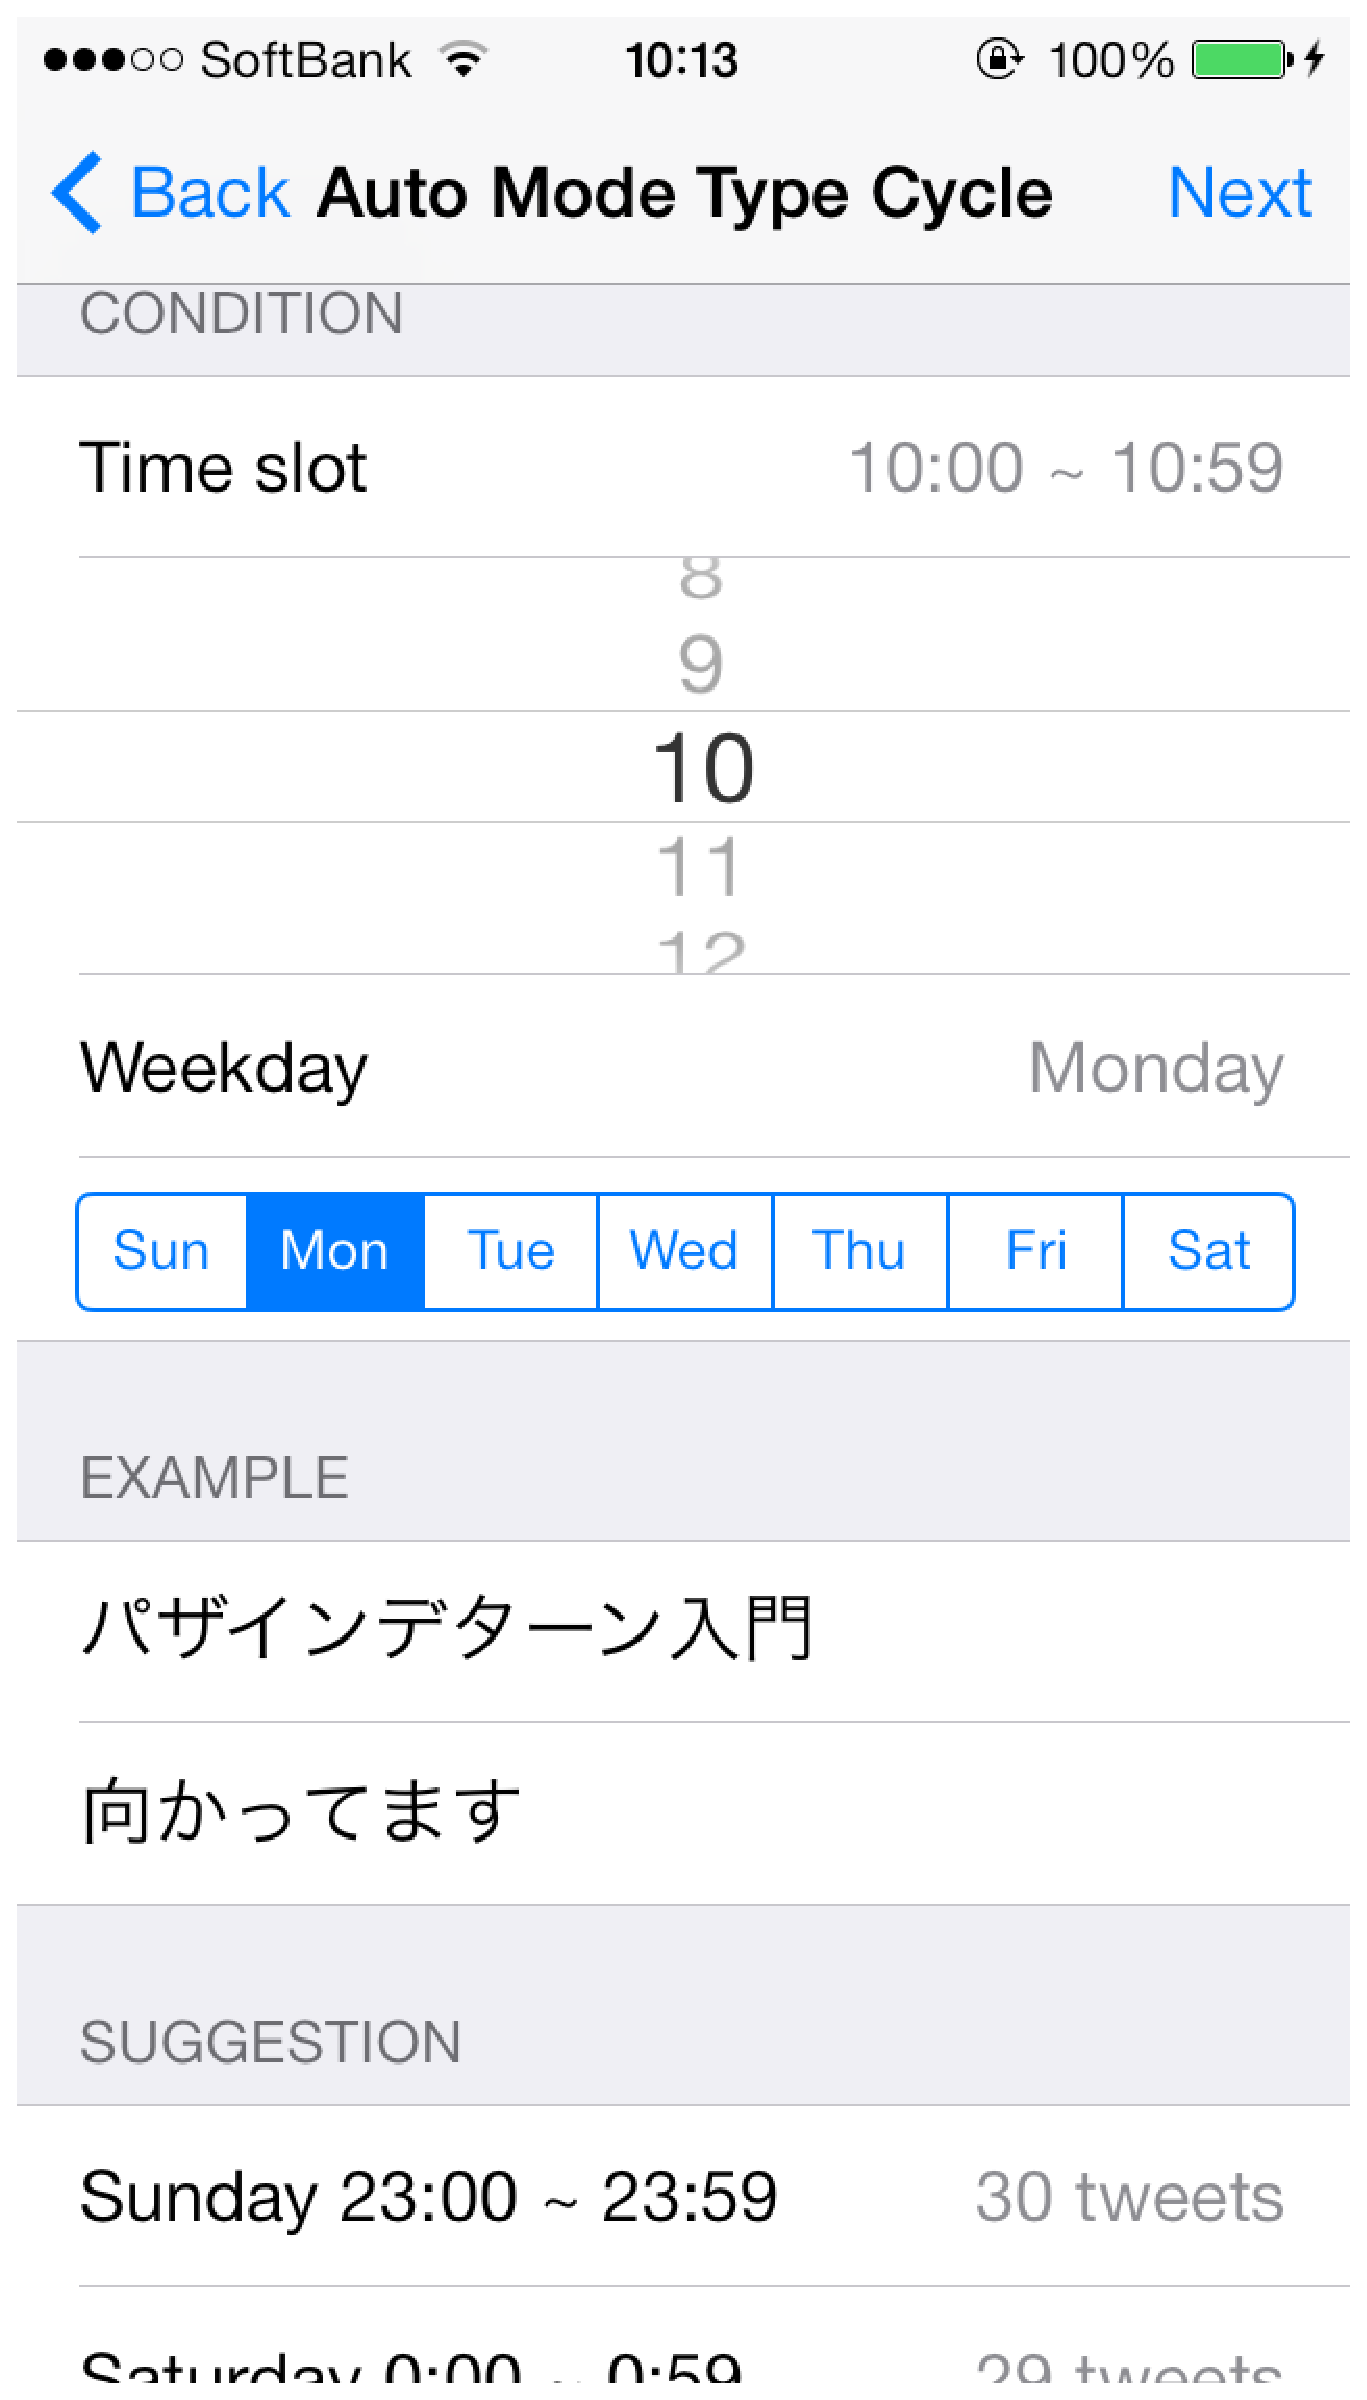
\includegraphics[width=60mm]{img/notifauthAutoCycle.eps}
\end{center}
\caption{Auto Mode Type Cycleの設定画面}
\label{fig:notifauthAutoCycle}
\end{minipage}
\end{figure}

次に,各設定方法の概要を説明する.

Auto Mode Type Termでは,画面上段の「CONDITION」においてスライダーを用いて「From」(どのくらい前のツイートから秘密情報とするか)と「Term」(Fromからどのくらいの期間のツイートを秘密情報とするか)を設定する.
各スライダーの最大値は,Notifauthによって取得しデータベースに保持されているツイートの中から最も古いものを基準として用いる.
また,画面下段の「EXAMPLE」に,秘密情報として該当するツイートの一部(1行目が最古のもの,3行目が最新のもの,2行目はツイート群の配列の中央値のもの)を表示し,ユーザの設定を補助する.

Auto Mode Type Cycleでは,画面上段の「CONDITION」においてピッカーを用いて「Time slot」(1時間単位で,何時のツイートを秘密情報とするか)を,セレクターを用いて「Weekday」(何曜日のツイートを秘密情報とするか)を設定する.
また,画面中断の「EXAMPLE」に,秘密情報として該当するツイートの一部(1行目が最古のもの,3行目が最新のもの,2行目はツイート群の配列の中央値のもの)を表示し,画面下段の「SUGGESTION」にはNotifauthによって取得しデータベースに保持されているツイートの中で投稿回数が多い曜日・時間の組み合わせを上位3つ表示する.
これらを参考にすることでユーザの設定を補助する.

\begin{figure}
\begin{center}
\includegraphics[width=60mm]{img/notifauthManual.eps}
\end{center}
\caption{Manual Modeの設定画面}
\label{fig:notifauthManual}
\end{figure}

Manual Modeでは,直近のツイートを最大200件取得し,これのうちどれを秘密情報とするかを手動で選択し設定する.
ここで設定したツイートは,もう一度設定しない限りは実験終了まで固定されたままである.

\subsection{認証操作}
認証操作としてiOSに実装されているロック画面上の通知とその選択操作(図\ref{fig:notificationSliding}\footnote{この場面ではスライドすることでロック解除後に受信したメールをすぐに読むことができる})を踏襲したものを採用した.
理由として,
\begin{enumerate}
\item 本システムは携帯端末における認証の多要素化を目指して実装され,その際開発環境であるiOSでそういった操作を行えるのはロック画面のみであったため
\item ロック画面で通知をスライドし選択する動作はiOS標準の機能であり,ユーザへ新たな操作を覚えさせる負担が少ないと考えたため
\end{enumerate}
が挙げられる.
また,実験を行いやすくするために本論文中の実装では,上記のロック画面を模した環境(図\ref{fig:notifauthNotificationTest},図\ref{fig:notifauthPINTest})をアプリケーション内に実装した.

\begin{figure}[ht]
\begin{center}
\epsfig{file=img/notificationSliding.eps,scale=0.35}
\end{center}
\caption{ロック画面上における通知の選択(スライド)動作の例}
\label{fig:notificationSliding}
\end{figure}

\begin{figure}[ht]
\begin{minipage}{0.5\hsize}
\begin{center}
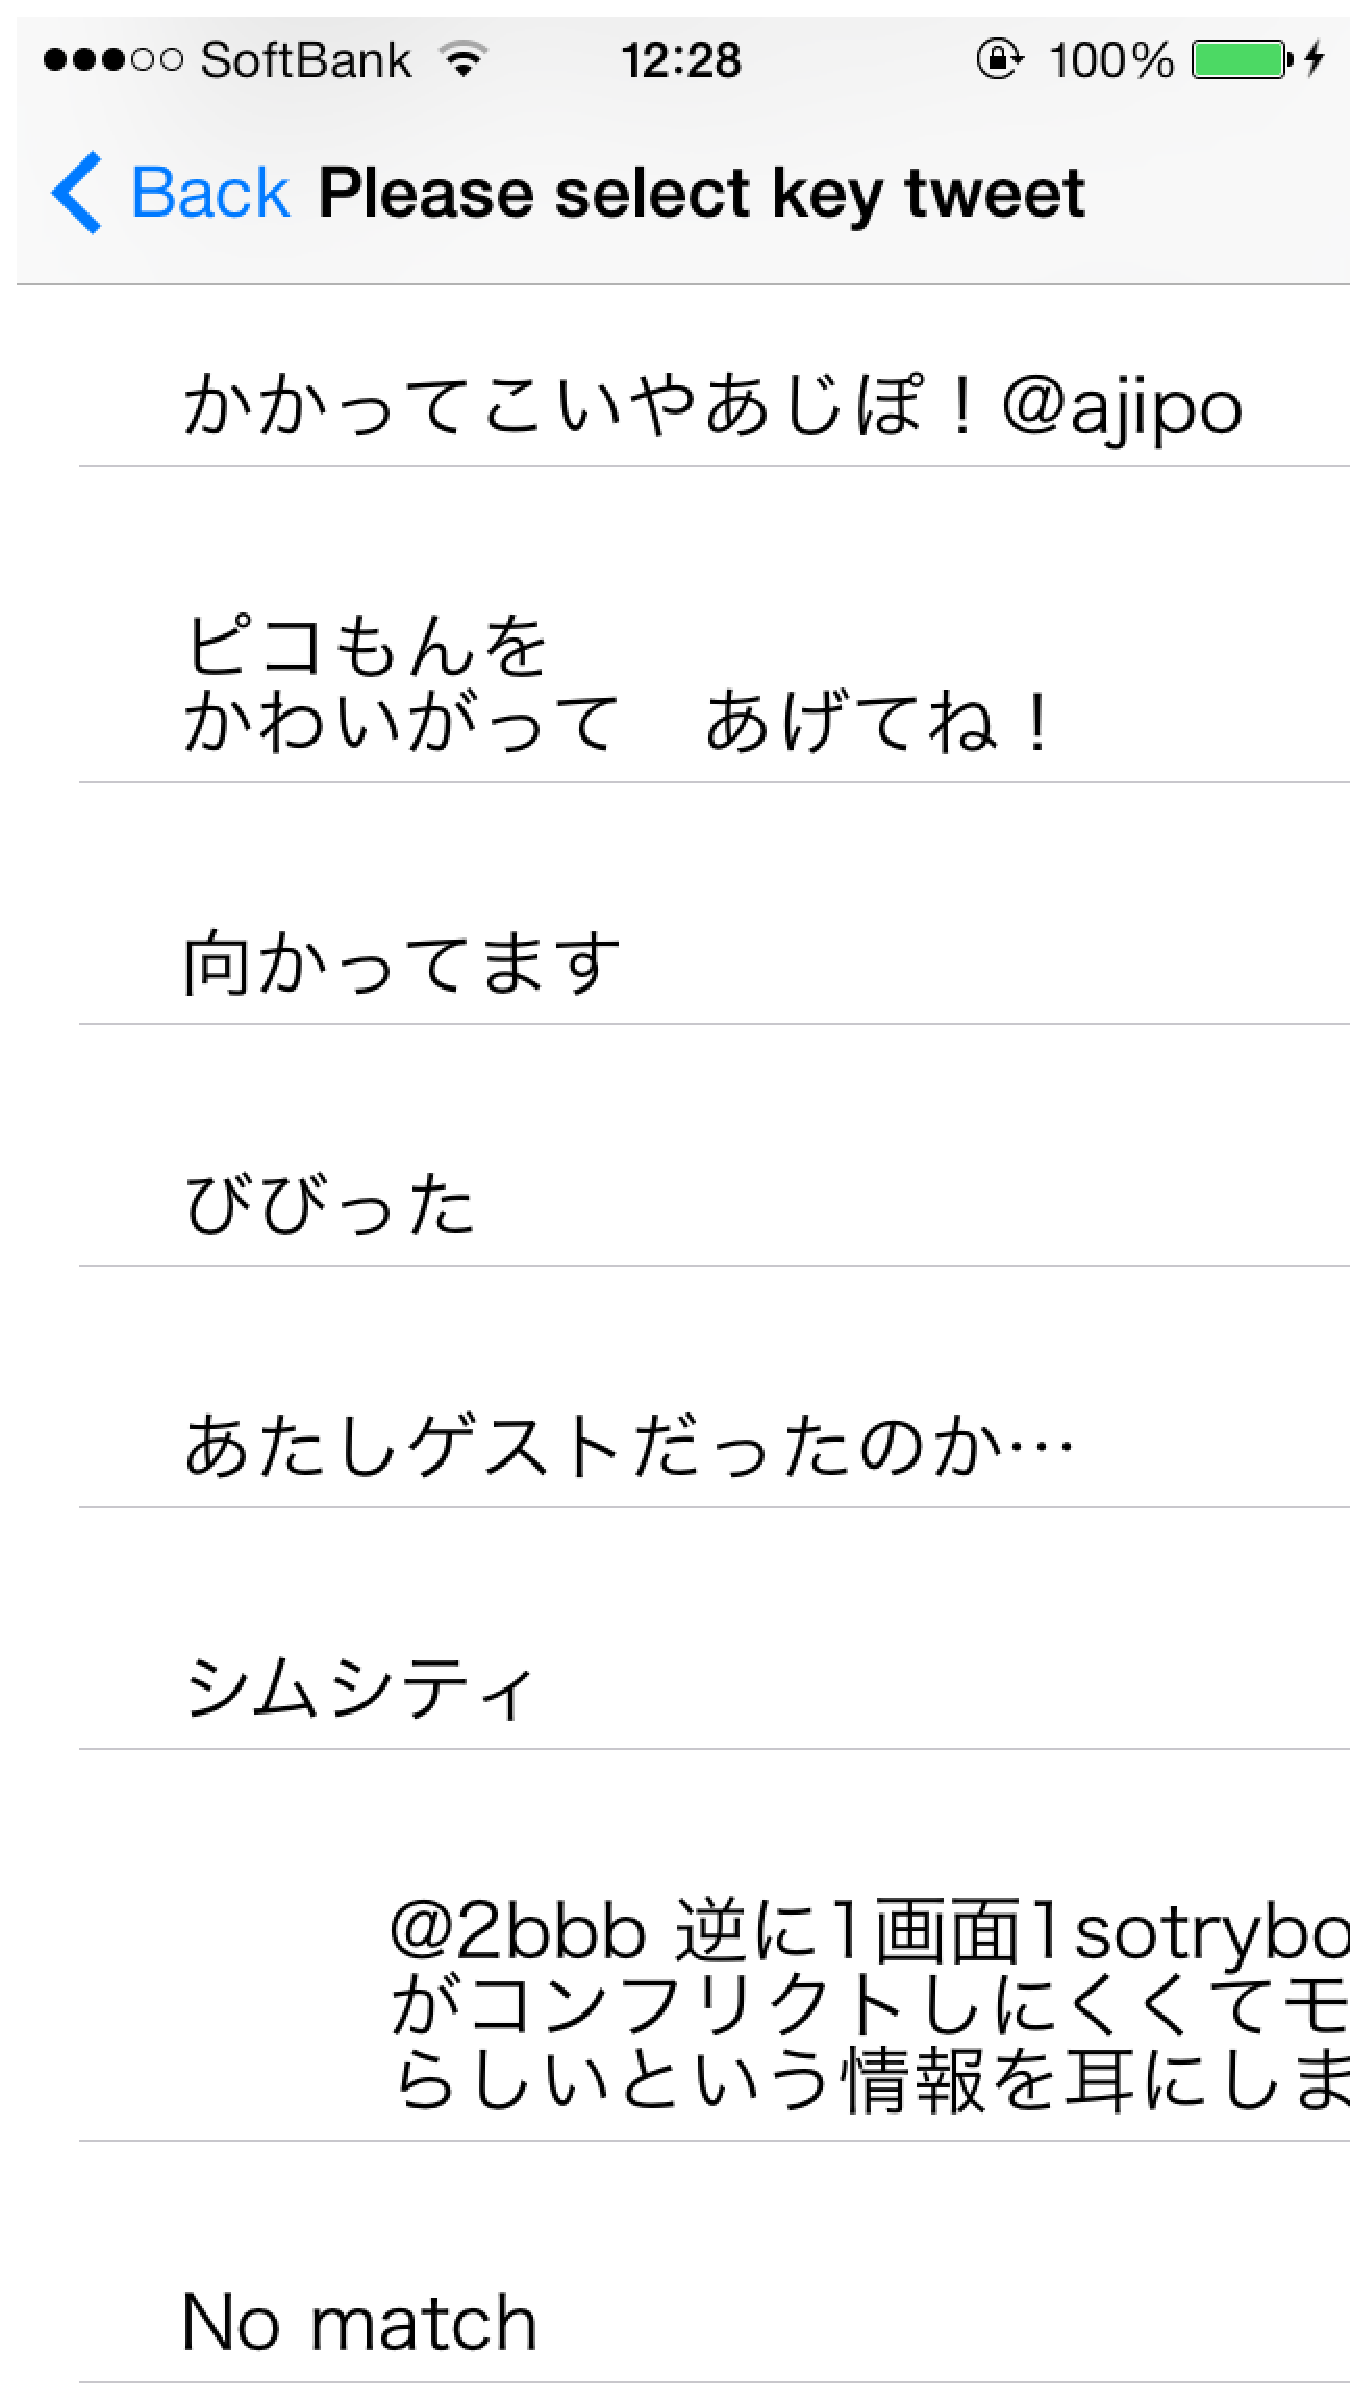
\includegraphics[width=60mm]{img/notifauthNotificationTest.eps}
\end{center}
\caption{ロック画面における通知の表示画面を模した認証画面}
\label{fig:notifauthNotificationTest}
\end{minipage}
\begin{minipage}{0.5\hsize}
\begin{center}
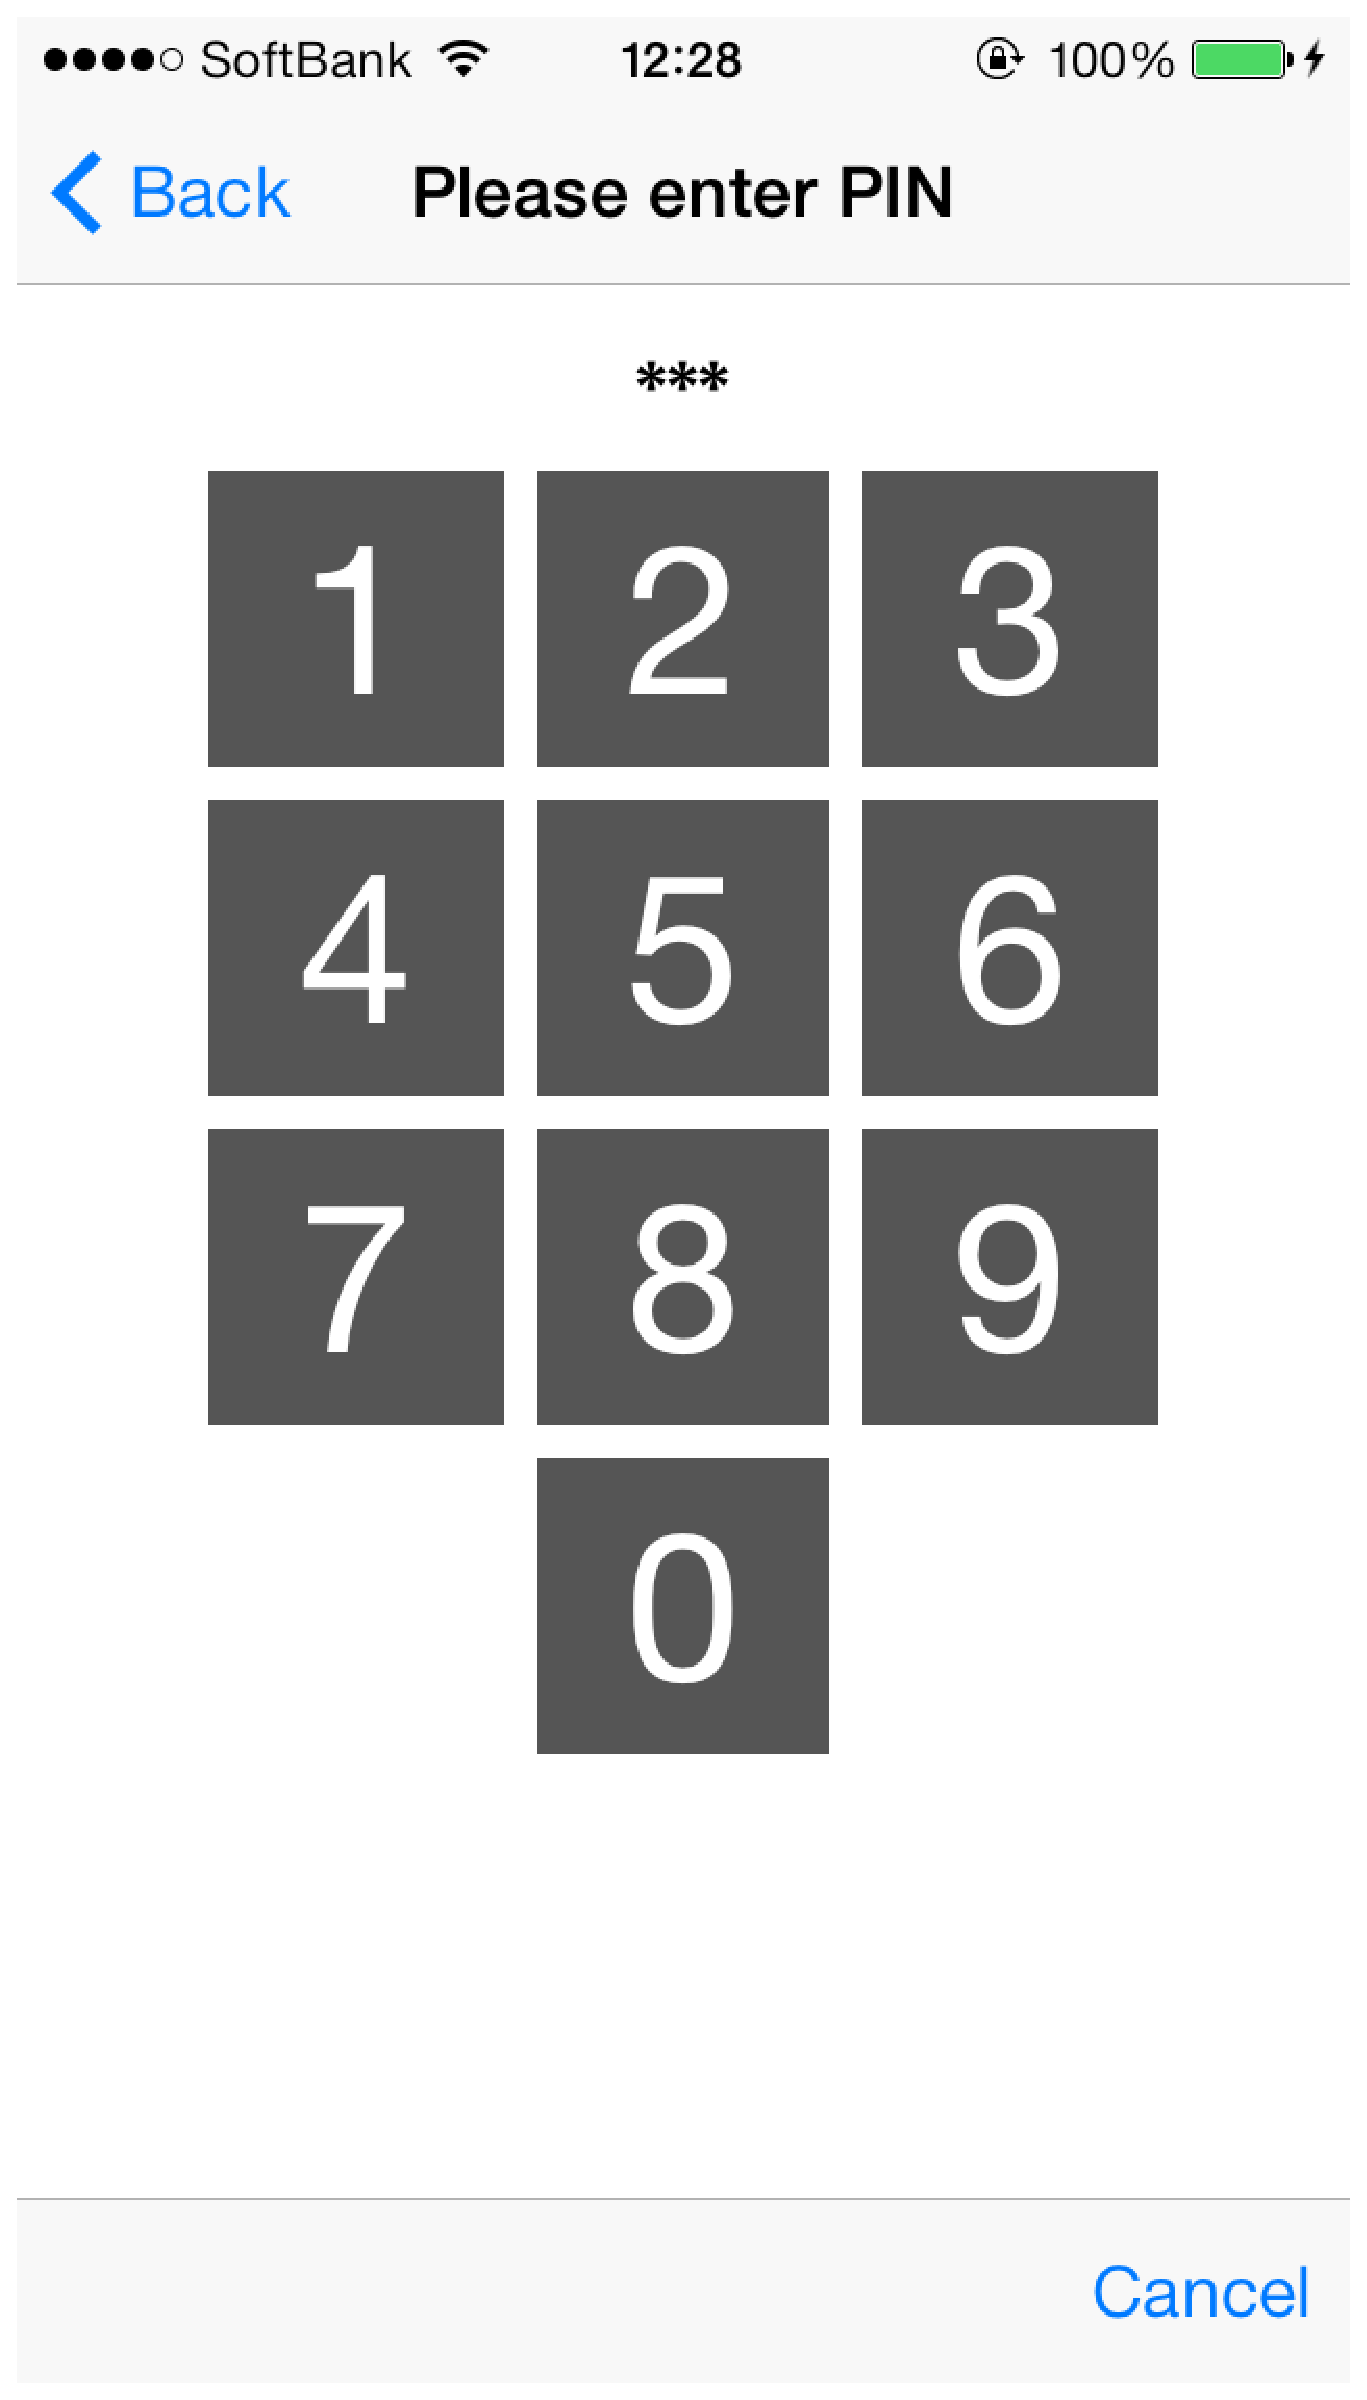
\includegraphics[width=60mm]{img/notifauthPINTest.eps}
\end{center}
\caption{ロック画面におけるPINの入力画面を模した認証画面}
\label{fig:notifauthPINTest}
\end{minipage}
\end{figure}

\subsection{前提条件}
\begin{table}[htpb]
\begin{center}
\caption{必要環境等}
\label{tbl:requirements}
\vspace{4mm}
\begin{tabular}{l||c|r}
必要条件 & iOS7を利用し,Twitterアカウントを保持していること \\
事前準備 & TwitterのOAuthを用いて本ソフトウェアと連携する \\
実装環境 & Mac OSX 10.9, Xcode5 \\
動作確認環境 & iPhone 4,iPhone 4S,iPhone 5,iPhone 5S,iPod touch \\
\end{tabular}
\end{center}
\end{table}

\section{具体的特徴}\label{sec:feature}
\subsection{時間経過による秘密情報の変化}
Auto Mode Type Termにおいて,設定を行った時から時間が経過すると秘密情報とするツイートが入れ替わる場合がある.
これが成立することの利点としては,
\begin{itemize}
\item 定期的な秘密情報の変更を能動的に行う必要が低減される
\item 設定した期間等が秘匿されている限り,出現頻度による攻撃がしにくくなる可能性がある
\end{itemize}
が挙げられる.

また,Auto Mode Type Cycleにおいては,
\begin{itemize}
\item 新たな秘密情報の候補が出現することで,統計的手法を用いた攻撃に対し強度が高くなる可能性がある
\end{itemize}
ということも利点として考えられる.

欠点としては以下のようなものが挙げられる.
\begin{itemize}
\item ユーザの本人認証率が下がる可能性がある
\item 期間の設定やツイートの頻度によっては,ダミーの数が減りすぎることで,統計的手法を用いた攻撃に脆弱になる恐れがある
\end{itemize}

本研究では,以上の利点が本当に作用するかどうかの検証実験も行った.

\newpage


%実験
\chapter{検証実験}\label{chap:experiment}

\section{概要}
本論文で提案する個人認証システムについて,3つの評価実験を行った.
それぞれの実験は,時間的な制約から予備実験,本実験などの形式で行うことをせず,一度に行った.

\subsection{実験手順}
以降の節のそれぞれの実験は第\ref{subsec:selectSecret}節にて挙げた3つの実装(以降,「パターン」と記載する)に対応しており,それぞれのパターンは多要素化手法として評価するために認証操作の後に4桁のPINによる認証操作を追加した.
そこに「PINの桁数を一桁増やし,5桁にしたものを秘密情報とする」パターンを追加し,計4パターンで相互に比較を行った.
各パターンの実験は一つにつき8日間にわたって実施,その間に設定した日から数えて,0日目(設定直後),1日目,3日目,8日目の4回の認証試行を行った.
それぞれのパターンで実験中の期間は重複せず,順番は偏りのないようにこちらで設定し,そのスケジュールにそって全実験を実施した.
スケジュールは4つのパターンの組み合わせであり,その総数は$ {}_4 P _4 $の式で表される.
本実験ではこれら全てに固有の番号(以降,「スケジュール番号」と記載する)を付録\ref{apdx:schedule}の通り割り振って管理する.

初回実験説明・導入
\begin{enumerate}
  \item 実験担当者が実験の目的・注意事項・免責事項を説明する.この手順は付録\ref{apdx:experiment}の実験説明資料と操作説明資料を用いておこなう.
  \item 不明な点があれば質問してもらう.
  \item 被験者のスケジュールを決定し,それに合わせて提案システムを実装したアプリケーションソフトウェア(以降「Notifauth」と記載する)のソースコードにスケジュール番号を登録する.
  \item 実験担当者の開発用端末と被験者の携帯端末を接続し,Appleの開発者用アカウントと被験者の端末の紐付けを行った上でNotifauthをインストールする.
  \item 実際にNotifauthを操作し,全てのパターンでひと通りの秘密情報設定と認証操作を行ってもらう.
  \item その後,Notifauth内の全ての保存されたデータを初期化し,スケジュールに沿ったパターンのみ設定を行ってもらうことで実験開始とする.
  \item 上記手順で設定したパターンについて認証操作を行ってもらう.
  \item この段階で実験データを送信してもらい,該当データの受信を実験担当者が確認ののち,初回実験説明・導入の終了とする.
\end{enumerate}

試行手順
\begin{enumerate}
  \item トップ画面で,試行したいパターンをセレクタで選択し,「Test」をタップする.
  \item ``PIN Mode''以外の場合,ロック画面を模した画面が表示され,秘密情報に当てはまると思われるツイートを見つけ,そのセルをスライドする.
  \item PINの入力画面が表示され,``PIN Mode''であれば5桁,それ以外のパターンであれば4桁のPINを入力する.
  \item 結果画面が表示されるので,「Home」をタップする.
\end{enumerate}

結果送信手順
\begin{enumerate}
  \item トップ画面で「Send」をタップすると,iOS標準のメール送信画面が開くので,何も編集を行わずに送信する.
  \item ここで仮にiOSへ自分のメール情報(送信サーバ,アカウントなど)が登録されていない場合以下の手順を行う
  \begin{enumerate}
    \item 「Send」をタップせず,トップ画面下部の「copy experiment data on clipboard」をタップする.
    \item クリップボードにデータがコピーされているので,メールアプリに貼り付けて実験担当者のメールアドレスへ送信する.
  \end{enumerate}
\end{enumerate}

\section{SNSの情報を利用することに関する評価実験}\label{sec:vsTweet}
\subsection{目的}
本実験では,SNSの情報を利用することで,従来のPINを一桁増やした認証と比較し,どれだけ利便性と安全性を向上させることができるかの評価を行う.
本実験で評価対象とするパターンとして,``Manual Mode''を採用する.

\subsection{方法}
付録の\ref{apdx:interimEnquete}や\ref{apdx:finalEnquete}にある通り,被験者には使用パターンについて5段階のリッカート尺度を使った質問に答えてもらい,さらに既に8日間の試行が終了している他パターンとの比較もしてもらう.

\subsection{結果}
(ここに最高の結果が入る)

\section{時系列における期間を秘密として用いることに関する評価実験}\label{sec:vsTerm}
\subsection{目的}
本実験では,SNSの情報の特性を利用した認証システムの記憶持続性と利便性の評価を行う.
また,他の実験で用いたパターンとの比較も行う.
本実験で評価対象とするパターンとして,``Auto Mode Type Term''を採用する.

\subsection{方法}
付録の\ref{apdx:interimEnquete}や\ref{apdx:finalEnquete}にある通り,被験者には使用パターンについて5段階のリッカート尺度を使った質問に答えてもらい,さらに既に8日間の試行が終了している他パターンとの比較もしてもらう.

\subsection{結果}
(ここに最高の結果が入る)

\section{時系列における周期を秘密として用いることに関する評価実験}\label{sec:vsCycle}
\subsection{目的}
本実験では,SNSの情報の特性を利用した認証システムの記憶持続性と利便性の評価を行う.
また,他の実験で用いたパターンとの比較も行う.
本実験で評価対象とするパターンとして,``Auto Mode Type Cycle''を採用する.

\subsection{方法}
付録の\ref{apdx:interimEnquete}や\ref{apdx:finalEnquete}にある通り,被験者には使用パターンについて5段階のリッカート尺度を使った質問に答えてもらい,さらに既に8日間の試行が終了している他パターンとの比較もしてもらう.

\subsection{結果}
(ここに最高の結果が入る)

\newpage


%考察
\chapter{考察}\label{chap:discussion}

\section{安全性に関する考察}\label{sec:safety}
安全性に関しては,単純な組み合わせにおいてはPINによる方式を上回り,さらにダミーの数を増やすことで柔軟に安全性を高めることができる.更に,hogeによりhageといったことが考えられる.しかし,設定情報をいかに秘匿するかといった面では,暗号化などの改善を行う必要がある.

\section{憶えやすさに関する考察}\label{sec:memorable}
本システムの認証方式では,Twitterの投稿を用いることによって憶えやすさを向上させることが主たる目的として存在した.
しかし,被験者実験において,秘密情報の設定方法によっては憶えやすさが低下するという結果が得られたため,ユーザの記憶が曖昧になってしまうと考えられる情報を排除するなどの対策をとる必要があると考えられる.

\section{使用継続性に関する考察}\label{sec:continuity}
本システムの認証方式では,設定方法によっては長期間使用することにより,秘密情報のエントロピーが上昇したり,自動的に秘密情報が入れ替わることで定期的な秘密情報変更をする必要が小さくなるなどの利点が存在する.また,被験者実験で得られた感想などから見ても,利便性についての評価が高いので,使用継続性が高いと考えられる.

\section{他環境における応用に関する考察}\label{sec:application}
本システムの考え方は,ハードウェアへの依存の少なさや,設定の柔軟さから,携帯端末以外の環境でも応用が可能だと考えられる.
被験者実験にて実施したアンケートでは,「○○などに導入したい」といった意見を得ることができた.

\newpage


%結論
\chapter{結論}\label{chap:conclusion}
本論文では,Twitterの情報を用いた携帯端末向け個人認証の多要素化手法の提案,実験と結果の解析を行った.本論文で提案した3種類の個人認証手法では,従来の知識認証のメリットを生かしつつ,新たな特徴を併せ持った認証要素を,様々な部分で応用できると考えている.また,被験者実験によって問題点の洗い出しと,今後の方向性の手がかりを得ることができた.しかしながら,実験に関しては手法などに問題点が多かったため,更なる検証を重ねてゆくことが欠かせないと感じた.

開発した認証システムのプログラムは付録\ref{apdx:code}にある通り,Web上で公開されている.これらの成果物はMITライセンスの下で自由にご利用していただいて構わない.今後のより良い個人認証の開発に少しでも貢献できたなら幸運である.

\newpage

%謝辞
\begin{ackn}{}

本研究を進めるにあたって,1年間を通して丁寧な御指導,数々の御助言をしてくださった高田哲司准教授に厚く御礼申し上げます.

また,研究について数々の知識やアドバイスをいただいた,高田研究室の皆様に深く感謝いたします.

加えて,実装や実験について数多くの知見を与えて下さり,本論文についても様々なご指摘を下さいました石井通人さんと原田陽紗子さん,更に,本論文の校正をして下さいました安部草麻生さん,実験に協力して下さった方々に深く感謝の意を申し上げます.

最後に,不自由ない学生生活を支援してくれた両親に心から感謝致します.

\end{ackn}{}
\newpage
% LocalWords:  ackn

%参考文献
%\begin{thebibliography}{99}

%\bibliographystyle{plain}
\bibliographystyle{unsrt}
\bibliography{documents/bibtex}

%\end{thebibliography}



% 付録
%\appendix
\chapter{実装に関する付録}\label{apdx:app}
\section{実装の詳細}
%(実装に関しては〜のはなし.クラス図とか概略図を入れたほうがよさそう)
Notifauthは,iOS用アプリケーションとして実装された.
クラス図は図\ref{fig:notifauthClass}の通りである.

\begin{figure}[ht]
  \begin{center}
    \epsfig{file=img/notifauthClass.eps,scale=0.2}
  \end{center}
  \caption{Notifauthのクラス図}
  \label{fig:notifauthClass}
\end{figure}

Twitterの認証情報(OAuthの認証トークン)は,Apple社の``Keychain''により,暗号化し保存されている.
ツイートのデータは,Object-relational mapping(以降ORM)フレームワークであるCoreDataを用いてSQLiteファイルに保存されている.
また,Notifauth内の様々な設定情報はiOS標準のNSUserDefaultsオブジェクトを利用しアプリケーションソフトウェア内の専用領域に保存されており.今回は特に暗号化は行っていない.

使用したサードパーティ製ライブラリは
\begin{itemize}
\item MagicalRecord
\item MKNetworkKit
\item RSOAuthEngine
\item RSTwitterEngine
\item NSDate-Utilities
\end{itemize}
である.
ソースコードは付録\ref{apdx:code}にある通り,Webで一般公開されている.

\section{実装コード}\label{apdx:code}
Mac OSXのXcode 5上にて,Objective-Cを用いて実装した.
ソースコード等を含めたXcodeプロジェクトの各ファイルは,\url{https://github.com/storz/Notifauth}へ設置し,MITライセンスにより配布している.

\section{画面一覧}\label{apdx:screen}
\begin{figure}[ht]
  \begin{minipage}{0.5\hsize}
    \begin{center}
      \includegraphics[width=40mm]{img/notifauthHome.eps}
    \end{center}
    \caption{Notifauth起動時の画面}
    \label{fig:notifauthHome}
  \end{minipage}
  \begin{minipage}{0.5\hsize}
    \begin{center}
      \includegraphics[width=40mm]{img/notifauthLogin.eps}
    \end{center}
    \caption{Notifauthユーザ登録画面}
    \label{fig:notifauthLogin}
  \end{minipage}
\end{figure}

\begin{figure}[ht]
  \begin{minipage}{0.5\hsize}
    \begin{center}
      \includegraphics[width=40mm]{img/notifauthPIN.eps}
    \end{center}
    \caption{Notifauth設定時のPIN登録画面}
    \label{fig:notifauthPIN}
  \end{minipage}
  \begin{minipage}{0.5\hsize}
    \begin{center}
      \includegraphics[width=40mm]{img/notifauthResult.eps}
    \end{center}
    \caption{Notifauth認証終了時の画面}
    \label{fig:notifauthResult}
  \end{minipage}
\end{figure}

\chapter{実験に関する付録}\label{apdx:experiment}
\section{スケジュール番号}\label{apdx:schedule}
\begin{table}[ht]
  \begin{minipage}{0.5\hsize}
    \begin{center}
      \small
      \begin{tabular}{l|c} \hline
        スケジュール番号 & 順番 \\ \hline
        0 & A→B→C→D \\
        1 & A→B→D→C \\
        2 & A→C→B→D \\
        3 & A→C→D→B \\
        4 & A→D→B→C \\
        5 & A→D→C→B \\
        6 & B→A→C→D \\
        7 & B→A→D→C \\
        8 & B→C→A→D \\
        9 & B→C→D→A \\
        10 & B→D→A→C \\
        11 & B→D→C→A \\ \hline
      \end{tabular}
    \end{center}
  \end{minipage}
  \begin{minipage}{0.5\hsize}
    \begin{center}
      \small
      \begin{tabular}{l|c} \hline
        スケジュール番号 & 順番 \\ \hline
        12 & C→A→B→D \\
        13 & C→A→D→B \\
        14 & C→B→A→D \\
        15 & C→B→D→A \\
        16 & C→D→A→B \\
        17 & C→D→B→A \\
        18 & D→A→B→C \\
        19 & D→A→C→B \\
        20 & D→B→A→C \\
        21 & D→B→C→A \\
        22 & D→C→A→B \\
        23 & D→C→B→A \\ \hline
      \end{tabular}
    \end{center}
  \end{minipage}
\end{table}
\begin{description}
  \item[A]:Auto Mode Type Term
  \item[B]:Auto Mode Type Cycle
  \item[C]:Manual Mode
  \item[D]:PIN Mode
\end{description}

\section{結果送信の詳細手順}
\begin{enumerate}
  \item トップ画面で「Send」をタップすると,iOS標準のメール送信画面が開くので,何も編集を行わずに送信する.
  \item ここで仮にiOSへ自分のメール情報(送信サーバ,アカウントなど)が登録されていない場合以下の手順を行う
  \begin{enumerate}
    \item 「Send」をタップせず,トップ画面下部の「copy experiment data on clipboard」をタップする.
    \item クリップボードにデータがコピーされているので,メールアプリに貼り付けて実験担当者のメールアドレスへ送信する.
  \end{enumerate}
\end{enumerate}

\newpage

\section{評価実験の概要説明資料}
\includegraphics[width=14.3cm]{resource/intro_1.ps}
\newpage
\includegraphics[width=14.3cm]{resource/intro_2.ps}
\newpage

\section{Notifauth操作マニュアル}
\includegraphics[width=14.3cm]{resource/manual-page1.pdf}
\newpage
\includegraphics[width=14.3cm]{resource/manual-page2.pdf}
\newpage
\includegraphics[width=14.3cm]{resource/manual-page3.pdf}
\newpage
\includegraphics[width=14.3cm]{resource/manual-page4.pdf}
\newpage
\includegraphics[width=14.3cm]{resource/manual-page5.pdf}
\newpage
\includegraphics[width=14.3cm]{resource/manual-page6.pdf}
\newpage
\includegraphics[width=14.3cm]{resource/manual-page7.pdf}
\newpage
\includegraphics[width=14.3cm]{resource/manual-page8.pdf}
\newpage
\includegraphics[width=14.3cm]{resource/manual-page9.pdf}
\newpage

\section{評価実験における中間アンケート}\label{apdx:interimEnquete}
\includegraphics[width=14.3cm]{resource/enquete_interim_1.ps}
\newpage
\includegraphics[width=14.3cm]{resource/enquete_interim_2.ps}
\newpage
\includegraphics[width=14.3cm]{resource/enquete_interim_3.ps}
\newpage
\includegraphics[width=14.3cm]{resource/enquete_interim_4.ps}
\newpage
\includegraphics[width=14.3cm]{resource/enquete_interim_5.ps}
\newpage

\section{評価実験における最終アンケート}\label{apdx:finalEnquete}
\includegraphics[width=14.3cm]{resource/enquete_final-page1.pdf}
\newpage
\includegraphics[width=14.3cm]{resource/enquete_final-page2.pdf}
\newpage
\includegraphics[width=14.3cm]{resource/enquete_final-page3.pdf}
\newpage
\includegraphics[width=14.3cm]{resource/enquete_final-page4.pdf}
\newpage
\includegraphics[width=14.3cm]{resource/enquete_final-page5.pdf}
\newpage
\includegraphics[width=14.3cm]{resource/enquete_final-page6.pdf}
\newpage
\includegraphics[width=14.3cm]{resource/enquete_final-page7.pdf}
\newpage
\includegraphics[width=14.3cm]{resource/enquete_final-page8.pdf}
\newpage
\includegraphics[width=14.3cm]{resource/enquete_final-page9.pdf}
\newpage
\includegraphics[width=14.3cm]{resource/enquete_final-page10.pdf}
\newpage
\includegraphics[width=14.3cm]{resource/enquete_final-page11.pdf}
\newpage
\includegraphics[width=14.3cm]{resource/enquete_final-page12.pdf}
\newpage


%\addcontentsline{toc}{chapter}{索引}
%\printindex

\end{document}
